\documentclass{beamer}

\usepackage{microtype}
\usepackage{fontspec}
\usepackage{mathtools}
\usepackage{booktabs}
\usepackage{listings}


% \setmainfont{Source Sans Pro}
% \setsansfont[Scale=MatchLowercase]{Source Sans Pro}
% \setmonofont[Scale=MatchLowercase]{PragmataPro}

\title{Authorization Logic for Mobile Ecosystems}
\subtitle{Second Year Report}
\author{Joseph Hallett}
\date{13\textsuperscript{th} October 2015}

\begin{document}

\maketitle

\begin{frame}
  \begin{quote}
    Automatic tools and policy languages would
    provide a better means of enforcement for 
    mobile device policies than existing
    mechanisms which rely on manual inspection. 
  \end{quote}
\end{frame}


\begin{frame}
  \frametitle{AppPAL}
  \begin{itemize}
  \item Authorization language for \emph{app installation policies}
  \item Instantiation of \emph{Becker~et~al.'s SecPAL} in Java
  \item Glue between user and corporate \emph{device policies} and the
    \emph{static analysis tools} and \emph{trust relationships} used to
    implement them.
  \item Designed to model and enforce policies in \emph{mobile ecosystems}
  \end{itemize}
\end{frame}

\begin{frame}
  \frametitle{Mobile Ecosystems}
  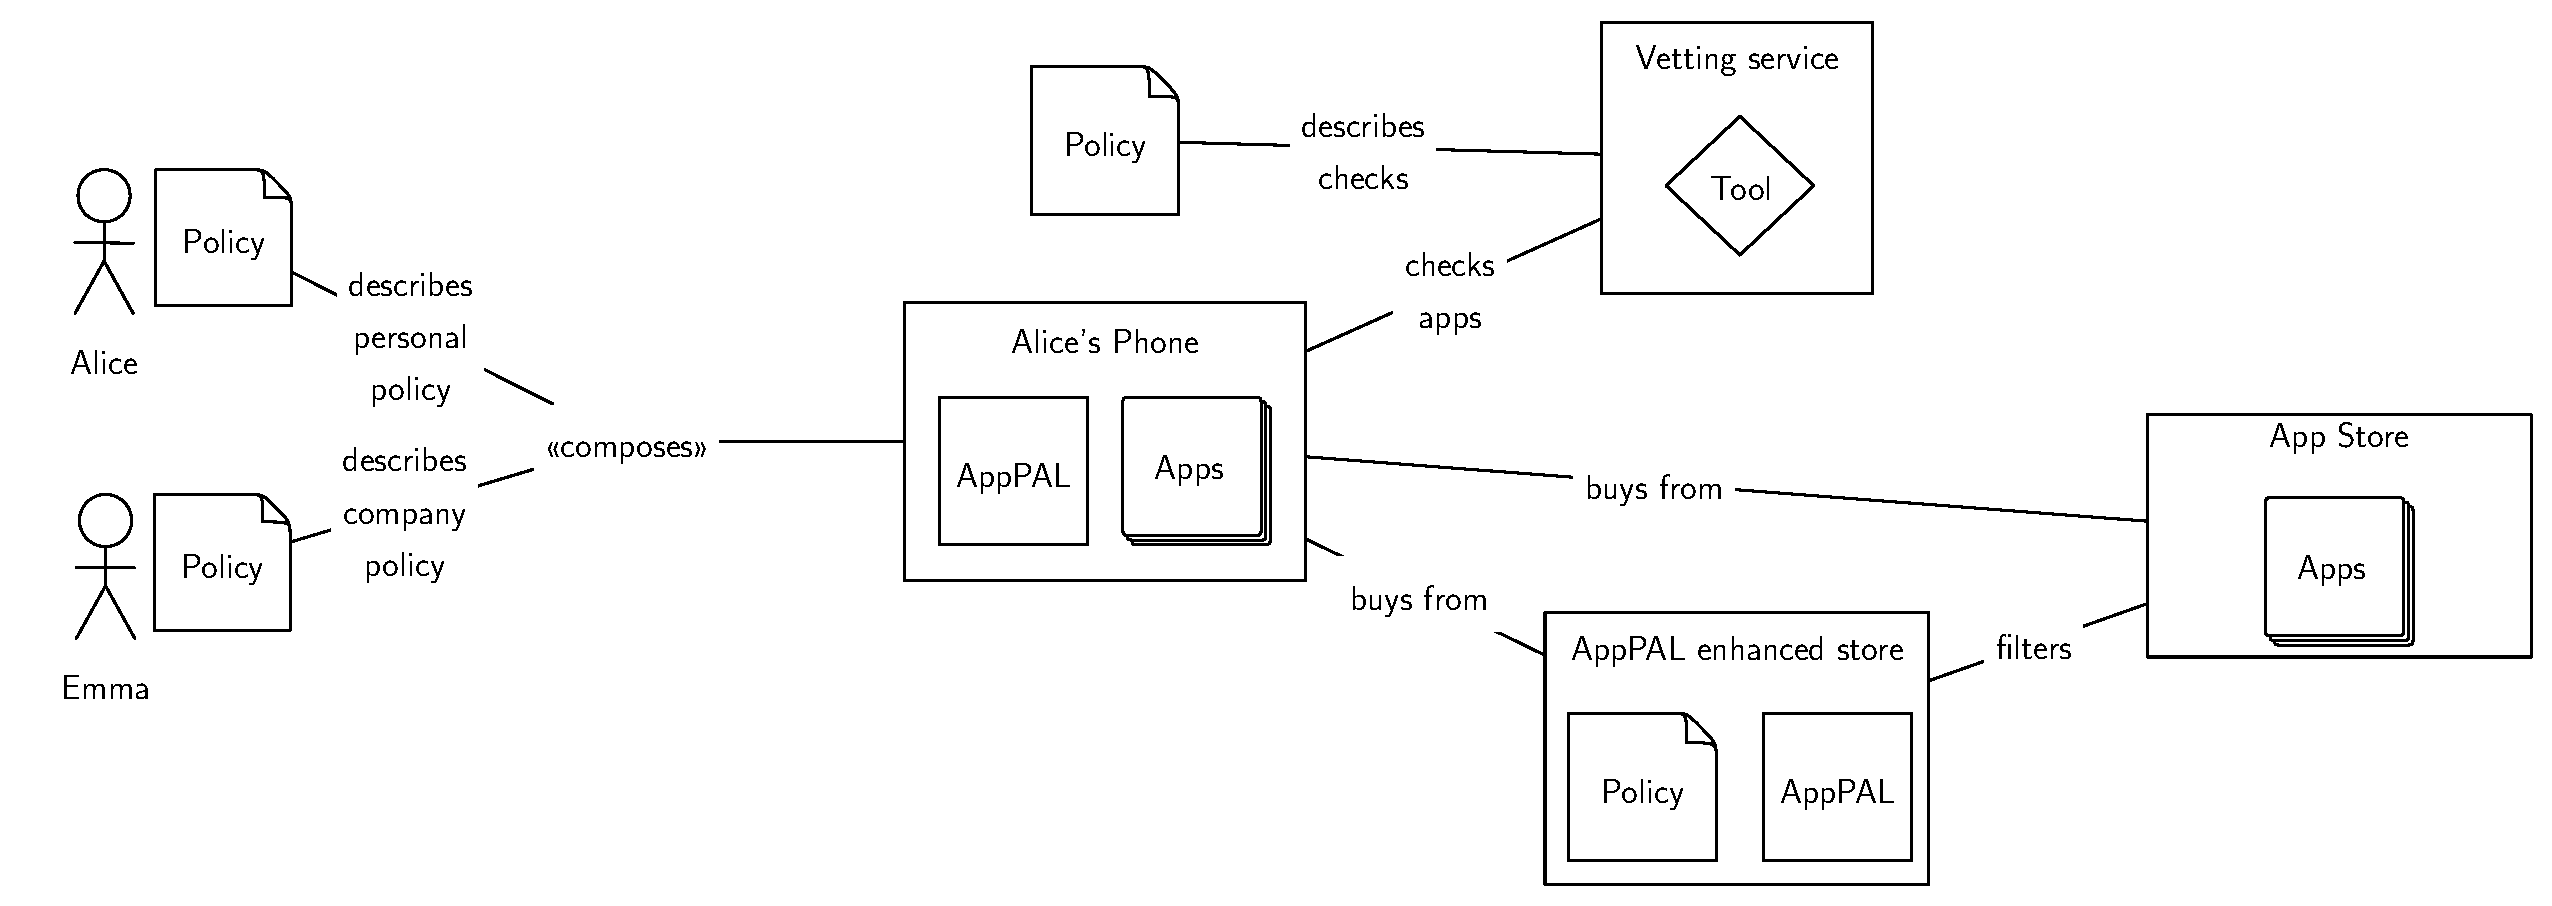
\includegraphics[width=\linewidth]{images/ecosystem.eps}
\end{frame}

\begin{frame}[fragile]
  \frametitle{AppPAL}
  \newcommand{\mybracetext}[1]{\text{\sffamily\footnotesize #1}}
  \newcommand{\mysmalltext}[1]{\text{\ttfamily\small #1}}
  
  \begin{center}
    \begin{equation*}
      \begin{array}{r l}
        \overbrace{\mysmalltext{'user'}}^{\mybracetext{speaker}}
        & \mysmalltext{ says }\overbrace{\overbrace{\mysmalltext{ App }}^{\mybracetext{subject}}\overbrace{\mysmalltext{ isRunnable}}^{\mybracetext{predicate}}}^{\mybracetext{fact}} \\
        & \overbrace{\mysmalltext{ if App isFree}}^{\mybracetext{condition}} \\
        & \overbrace{\mysmalltext{ where hasPermission(App, 'INTERNET') = True}}^{\mybracetext{constraint}}. \\
        \\        
        \mysmalltext{'user'}  
        & \mysmalltext{ says }\underbrace{\underbrace{\mysmalltext{'boss'}}_{\mybracetext{to}}\mysmalltext{ can-say }\underbrace{\mysmalltext{inf}}_{\mybracetext{depth}}\mysmalltext{App isInstallable.}}_{\mybracetext{delegation}}
      \end{array}
    \end{equation*}
  \end{center}
  
  % \newcommand{\nonterminal}[1]{{\small $\langle$#1$\rangle$}}
  % \newcommand{\terminal}[1]{{\small \texttt{#1}}}
  % \begin{center}
  %   \begin{tabular}{r c l}
  %     \nonterminal{Assertion} & $\coloneqq$ & \nonterminal{E} \terminal{says} \nonterminal{Fact} \\
  %                             &             & \hspace{1em}(\terminal{if} (\nonterminal{Fact}\terminal{,})+)?\terminal{.} \\
  %                             &             & \hspace{1em}(\terminal{where} \nonterminal{Constraint})? \\
  %     \nonterminal{Fact}      & $\coloneqq$ & \nonterminal{E} (\terminal{isRunable} $\vert$ $\ldots$) \\
  %                             & $\vert$     & \nonterminal{E} \terminal{can-say} \terminal{inf}? \nonterminal{Fact} \\
  %                             & $\vert$     & \nonterminal{E} \terminal{can-act-as} \nonterminal{E} \\
  %     \nonterminal{E}         & $\coloneqq$ & \terminal{Variable} $\vert$ \terminal{`constant'}
  %   \end{tabular}
  % \end{center}

\end{frame}

\begin{frame}[fragile]
  \frametitle{Example AppPAL Policy}
  \begin{center}
  \begin{lstlisting}[columns=flexible,basicstyle=\ttfamily\footnotesize]
'user' says App isInstallable
  if App hasCategory('game')
     App isGood
  where hasPermission(App, 'IAP') = False.

'user' says 'play-store' can-say App hasCategory(Category) 

'user' says 'review-site' can-say inf App isGood.

'review-site' says App isGood
  where reviewSiteScore(App) > 7.
  \end{lstlisting}
  \end{center}
\end{frame}

\begin{frame}
  \frametitle{Summary of Second Year Work}
  \begin{itemize}
    \item Created a knowledge base about android apps
    \item Implemented AppPAL on Android
    \item Explored the usage policies in current app stores
    \item Looked at the distribution mechanisims in current app stores
    \item Looked at the extent privacy preferences are being followed by users
      using current mechanisms
  \end{itemize}
\end{frame}

\begin{frame}
  \frametitle{Security Knowledge Base}
  \begin{itemize}
  \item Needed a knowledge base to store and collect metadata about apps
  \item Existing tooling overly complex and couldn't be extended (easily)
  \item Collects metadata for around 40,000 apps
  \item Can run static analysis tools on the apps and collect results
  \item Can output AppPAL statements
  \item Would be nice to keep extending and to query it from AppPAL
  \end{itemize}
\end{frame}

\begin{frame}
  \frametitle{AppPAL on Android}
  \begin{columns}
    \begin{column}{0.5\linewidth}
      \begin{itemize}
      \item Prototype from first year couldn't run on Android
      \item Reimplemented as a library for Java
      \item Created apps to scan installed apps against policies, create app
        stores with policies.
      \end{itemize}
    \end{column}
    \begin{column}{0.5\linewidth}\centering
      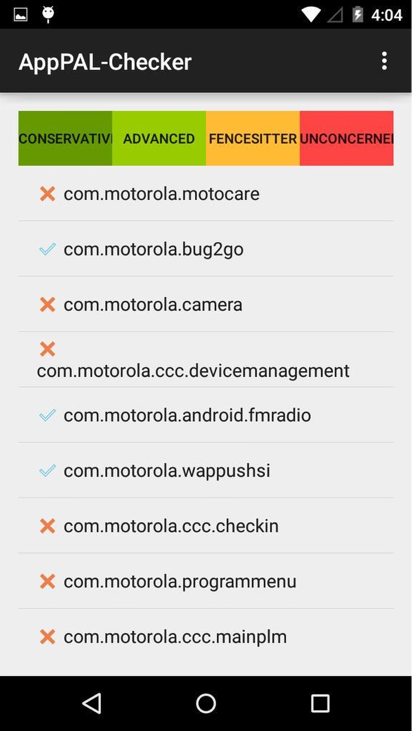
\includegraphics[width=0.7\linewidth]{images/apppal-checker.png}
    \end{column}
  \end{columns}
\end{frame}

\begin{frame}
  \frametitle{Policies in Current Stores}
  \begin{itemize}
  \item Looked at the developer and user terms of use for 4 different app
    markets
    \begin{itemize}
    \item Google Play, Amazon, Yandex and Aptoide
    \end{itemize}
  \item The policies are quite similar.
  \item Largest differences are to do with payment processing and age of use.
  \item Some stores keep modification rights
    \begin{itemize}
    \item Moves trust from developer to store
    \end{itemize}
  \end{itemize}
\end{frame}

\begin{frame}
  \frametitle{Distribution Mechanisms}
  \begin{columns}
    \begin{column}{0.5\linewidth}
      \begin{itemize}
      \item Used an SSL proxy to look at how the stores download apps
      \item Lots of implementation differences
      \item Some implementation problems
        \begin{itemize}
        \item Certificate pinning
        \item Encryption being dropped (or missing) for download
        \item Being able to re-download apps
        \end{itemize}
      \end{itemize}
    \end{column}
    \begin{column}{0.5\linewidth}
      \begin{center}
        \begin{tabular}{rrc}
          \toprule
          1. & $C \longrightarrow S$:        & $U, C, a_{\text{d}} $  \\ \addlinespace
          2. & $S \longrightarrow C$:        & $a_{\text{d}}, ? $     \\ \addlinespace
          3. & $C \longrightarrow S$:        & $U, ! $                \\ \addlinespace
          4. & $S \longrightarrow C$:        & $a_{\text{d}}, \$ $    \\ \addlinespace
          5. & $C \longrightarrow S$:        & $U, a_{\text{d}}, \$ $ \\ \addlinespace
          6. & $S \longrightarrow C$:        & $S^\prime$             \\ \addlinespace
          7. & $C \longrightarrow S^\prime$: &                        \\ \addlinespace
          8. & $S^\prime \longrightarrow C$: & $a$                    \\
          \bottomrule
        \end{tabular}
      \end{center}
    \end{column}
  \end{columns}
\end{frame}

\begin{frame}
  \frametitle{Policies in Practice}
  \begin{itemize}
  \item Using \emph{Carat} installation data we found 44,000 users for whom we
    new at least 20 apps they had installed
  \item Described 4 user privacy preference policies (\emph{Lin~et~al.}) using
    AppPAL
  \item Took a list of Android malware from McAfee and created \emph{no-malware} policies
  \item Ran \emph{MalloDroid} on the apps and created \emph{no-SSL-error} policies
  \item Measured the extent each user was following each policy 
  \end{itemize}
\end{frame}

\begin{frame}
  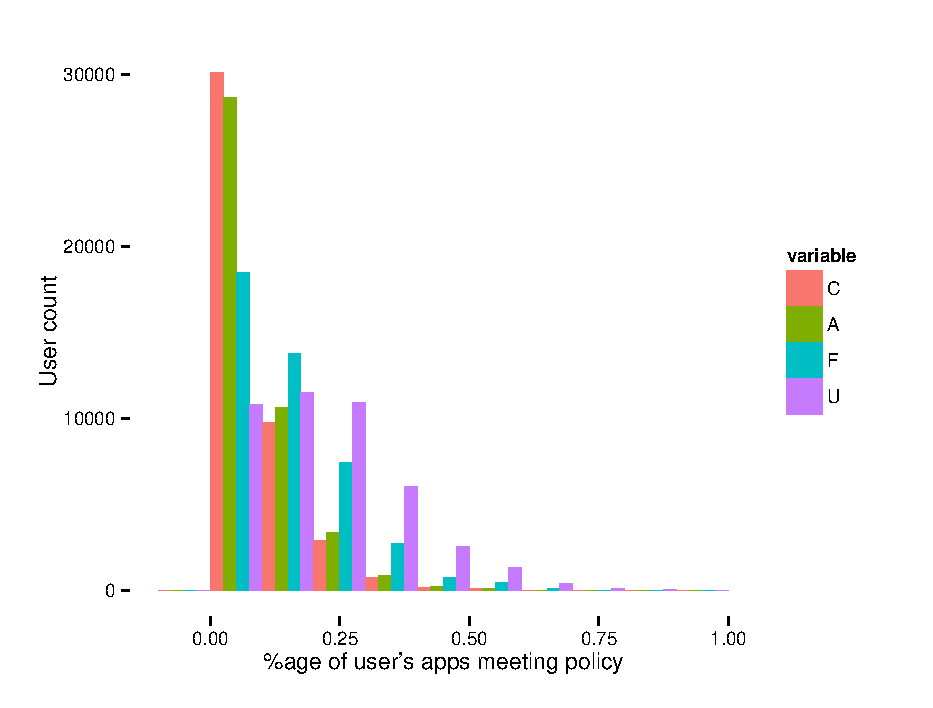
\includegraphics[width=\linewidth]{presentation/lin.eps}
\end{frame}
\begin{frame}
  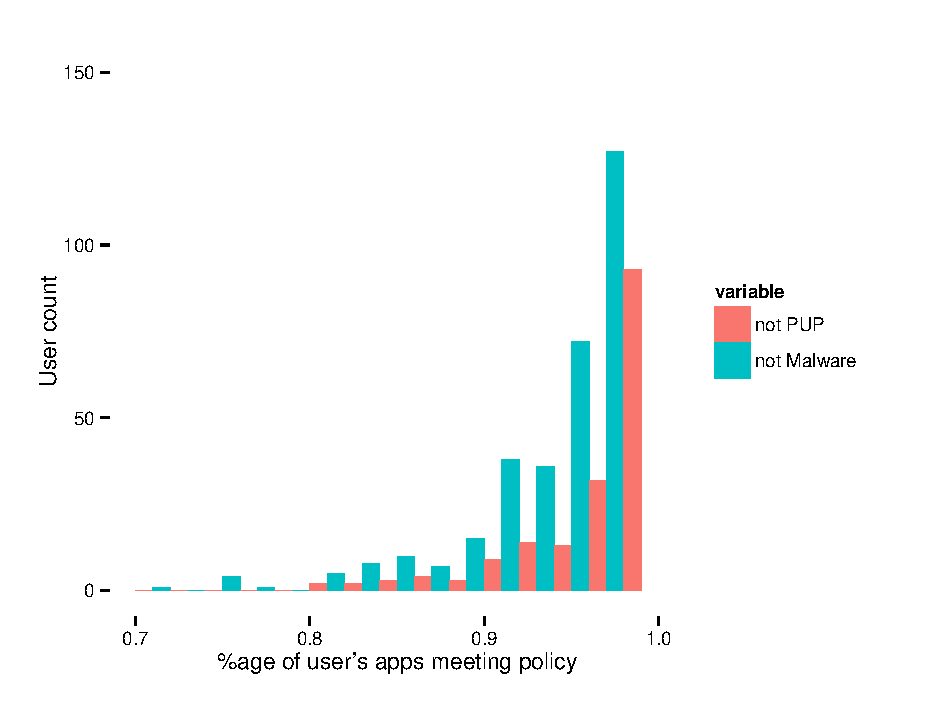
\includegraphics[width=\linewidth]{presentation/malware.eps}
\end{frame}
\begin{frame}
  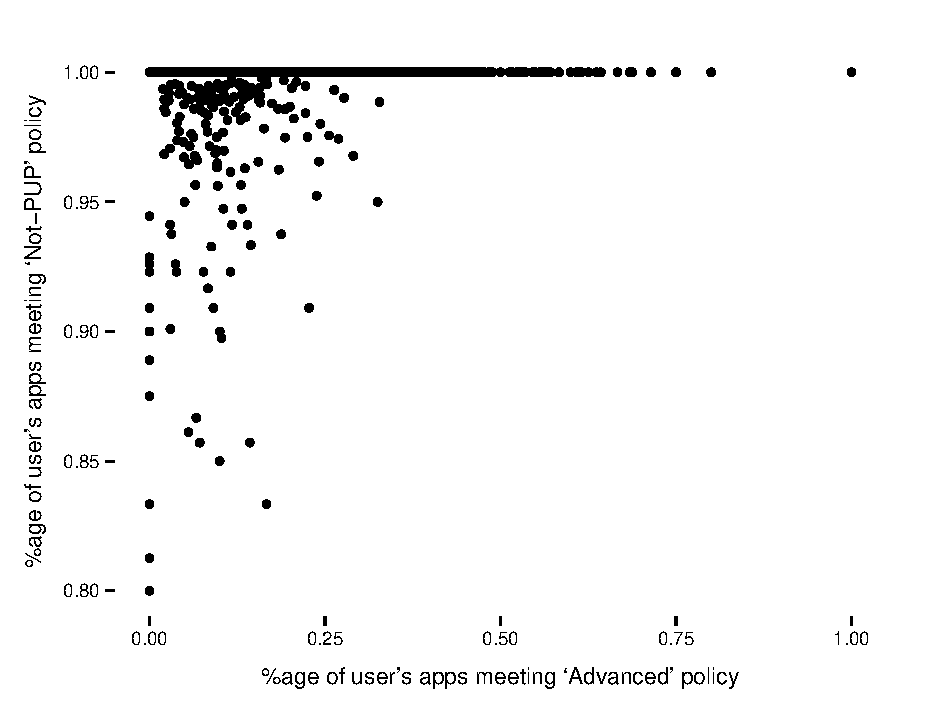
\includegraphics[width=\linewidth]{presentation/advanced-v-pup.eps}
\end{frame}
\begin{frame}
  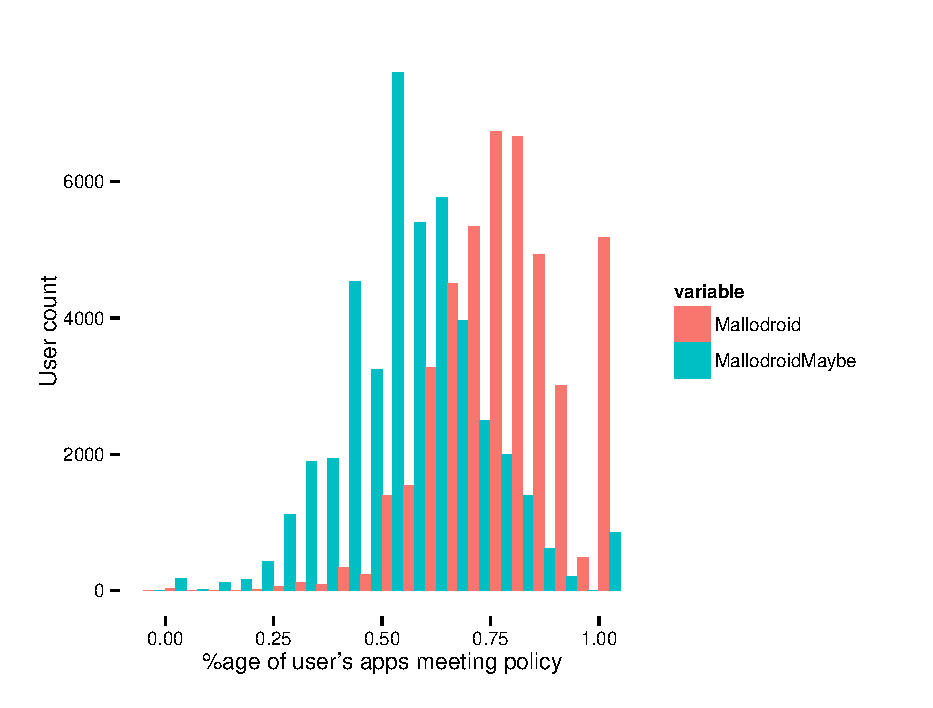
\includegraphics[width=\linewidth]{presentation/mallodroid.eps}
\end{frame}
\begin{frame}
  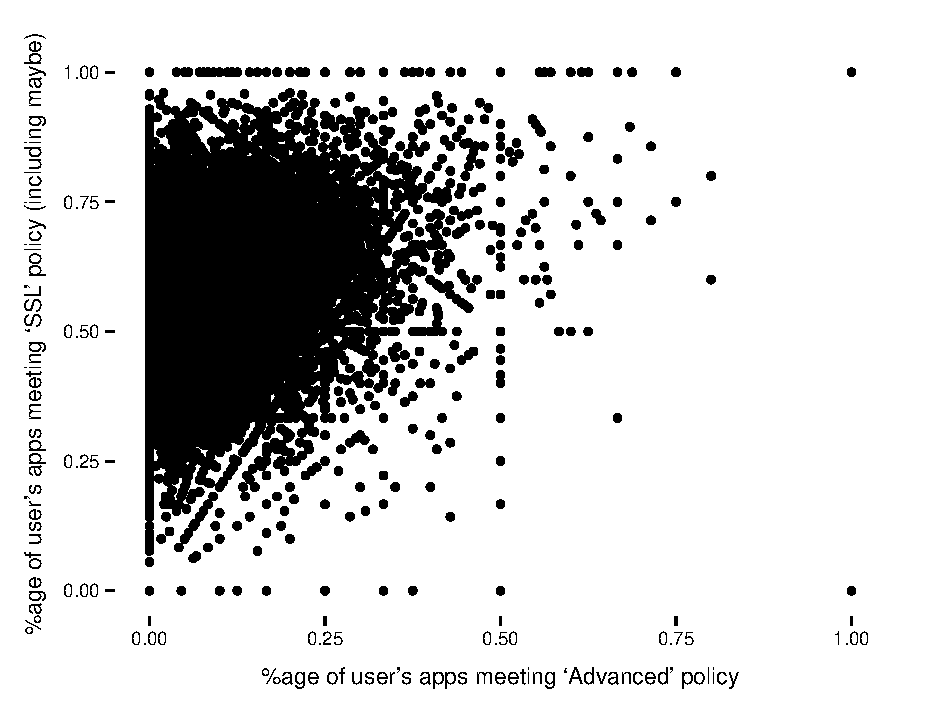
\includegraphics[width=\linewidth]{presentation/advanced-v-mallodroid_m.eps}
\end{frame}


\begin{frame}
  \frametitle{Proposed Third Year Work}
  \begin{itemize}
  \item Knowledge distribution protocols
  \item Case study with AppPAL
  \end{itemize}
\end{frame}

\begin{frame}
  \frametitle{Knowledge Distribution Protocols}
  \begin{itemize}
  \item We can express delegation relationships with SecPAL based languages
  \item It isn't clear how we should ask for more information
  \item Don't want delegatee to make the decision, necessarily
  \item Links to multi-agent knowledge distribution? (FIPA/KQML?)
  \end{itemize}
  \begin{itemize}
  \item A contribution to make AppPAL more distinct from SecPAL
  \item Links up with security knowledge base as a source of AppPAL statements
  \item How do we handle timely queries?
  \item How do we distinguish:
    \begin{itemize}
    \item not knowing
    \item not wanting to answer (because it's false)
    \item not wanting to answer (because they're unsure)
    \end{itemize}
  \item Could lead to questions whether we can quantify the trust we have in AppPAL statements?  
  \end{itemize}
\end{frame}

\begin{frame}
  \frametitle{Case Study}
  \begin{itemize}
  \item BYOD policies increasingly described informally by businesses
  \item Would like to implement one in AppPAL
    \begin{itemize}
    \item alternately NIST-SP-800--46/124
    \end{itemize}
    \item Shows the extent of what we can express in AppPAL
    \item Bigger use case than the hypothetical, and supposed, policies we've
      used so far
    \item May lead to other questions:
      \begin{itemize}
      \item Can policies be composed?
      \item What happens when multiple corporate policies disagree?
      \item What happens when policies change over time?
      \end{itemize}
  \end{itemize}
\end{frame}

\begin{frame}
  \frametitle{Questions?}
  
\end{frame}
\end{document}
% Local Variables:
% TeX-engine: xetex
% End:
